%-----------------------------------------------------------------------
%
%   UFRJ  - Universidade Federal do Rio de Janeiro
%   COPPE - Coordenação dos Programas de Pós-graduação em Engenharia
%   PEE   - Programa de Engenharia Elétrica
%
%
%   Projeto EMMA - 
%
%                                                        19/out/15, Rio
%                                                        Estevão F. Ferrão
%----------------------------------------------------------------------
%
%  Compilar usando PDFLaTeX
%
%----------------------------------------------------------------------
\documentclass[12pt,a4paper]{article}
\usepackage{macros/ROSApackages}
\usepackage[brazilian]{babel}

%-----------------------------------------------------------------------
%
%   UFRJ  - Universidade Federal do Rio de Janeiro
%   COPPE - Coordena��o dos Programas de P�s-gradua��o em Engenharia
%   PEE   - Programa de Engenharia El�trica
%
%
%   Projeto ROSA - Rob� para opera��o de stoplogs alagados
%
%   Settings
%                                                         Ramon R. Costa
%                                                         20/mar/14, Rio
%-----------------------------------------------------------------------

%---------------------------------------------------------- COLORS -----
%--------------------------------------------------- Bright colors -----
\definecolor{brightred}     {rgb}{1.00, 0.95, 0.95}
\definecolor{brightgreen}   {rgb}{0.95, 1.00, 0.95}
\definecolor{brightblue}    {rgb}{0.95, 0.95, 1.00}

\definecolor{brightyellow}  {rgb}{1.00, 1.00, 0.95}
\definecolor{brightmagenta} {rgb}{1.00, 0.95, 1.00}
\definecolor{brightcyan}    {rgb}{0.95, 1.00, 1.00}

\definecolor{brightorange}  {rgb}{1.00, 0.95, 0.85}

%----------------------------------------------------- Pale colors -----
\definecolor{palered}     {rgb}{1.00, 0.85, 0.85}
\definecolor{palegreen}   {rgb}{0.85, 1.00, 0.85}
\definecolor{paleblue}    {rgb}{0.85, 0.85, 1.00}

\definecolor{paleyellow}  {rgb}{1.00, 1.00, 0.85}
\definecolor{palemagenta} {rgb}{1.00, 0.85, 1.00}
\definecolor{palecyan}    {rgb}{0.85, 1.00, 1.00}

\definecolor{paleorange}  {rgb}{1.00, 0.85, 0.65}

%---------------------------------------------------- Light colors -----
\definecolor{lightred}     {rgb}{0.95, 0.00, 0.00}
\definecolor{lightgreen}   {rgb}{0.00, 0.95, 0.00}
\definecolor{lightblue}    {rgb}{0.00, 0.00, 0.95}

\definecolor{lightyellow}  {rgb}{0.95, 0.95, 0.00}
\definecolor{lightmagenta} {rgb}{0.95, 0.00, 0.95}
\definecolor{lightcyan}    {rgb}{0.00, 0.95, 0.95}

\definecolor{lightgray}    {rgb}{0.95, 0.95, 0.95}

\definecolor{lightorange}  {rgb}{0.95, 0.63, 0.00}

%--------------------------------------------------- Middle colors -----
\definecolor{midred}     {rgb}{0.85, 0.00, 0.00}
\definecolor{midgreen}   {rgb}{0.00, 0.85, 0.00}
\definecolor{midblue}    {rgb}{0.00, 0.00, 0.85}

\definecolor{midyellow}  {rgb}{0.85, 0.85, 0.00}
\definecolor{midmagenta} {rgb}{0.85, 0.00, 0.85}
\definecolor{midcyan}    {rgb}{0.00, 0.85, 0.85}

\definecolor{midgray}    {rgb}{0.85, 0.85, 0.85}

\definecolor{midorange}  {rgb}{0.85, 0.57, 0.00}

%--------------------------------------------------- Normal colors -----
\definecolor{red}     {rgb}{0.75, 0.00, 0.00}
\definecolor{green}   {rgb}{0.00, 0.75, 0.00}
\definecolor{blue}    {rgb}{0.00, 0.00, 0.75}

\definecolor{yellow}  {rgb}{0.75, 0.75, 0.00}
\definecolor{magenta} {rgb}{0.75, 0.00, 0.75}
\definecolor{cyan}    {rgb}{0.00, 0.75, 0.75}

\definecolor{gray}    {rgb}{0.75, 0.75, 0.75}

\definecolor{orange}  {rgb}{0.75, 0.50, 0.00}

%--------------------------------------------------- Shadow colors -----
\definecolor{shadred}     {rgb}{0.65, 0.00, 0.00}
\definecolor{shadgreen}   {rgb}{0.00, 0.65, 0.00}
\definecolor{shadblue}    {rgb}{0.00, 0.00, 0.65}

\definecolor{shadyellow}  {rgb}{0.65, 0.65, 0.00}
\definecolor{shadmagenta} {rgb}{0.65, 0.00, 0.65}
\definecolor{shadcyan}    {rgb}{0.00, 0.65, 0.65}

\definecolor{shadgray}    {rgb}{0.65, 0.65, 0.65}

\definecolor{shadorange}  {rgb}{0.65, 0.43, 0.00}

%--------------------------------------------------- Darker colors -----
\definecolor{darkred}     {rgb}{0.50, 0.00, 0.00}
\definecolor{darkgreen}   {rgb}{0.00, 0.50, 0.00}
\definecolor{darkblue}    {rgb}{0.00, 0.00, 0.50}

\definecolor{darkyellow}  {rgb}{0.50, 0.50, 0.00}
\definecolor{darkmagenta} {rgb}{0.50, 0.00, 0.50}
\definecolor{darkcyan}    {rgb}{0.00, 0.50, 0.50}

\definecolor{darkgray}    {rgb}{0.50, 0.50, 0.50}

\definecolor{darkorange}  {rgb}{0.50, 0.33, 0.00}

%-------------------------------------------------- Hyperref setup -----
\hypersetup{
  breaklinks   = true,
  colorlinks   = true,
  linkcolor    = darkblue,
  anchorcolor  = darkcyan,
  citecolor    = darkred,
  filecolor    = darkorange,
  menucolor    = darkmagenta,
  urlcolor     = darkgreen,
  pdfhighlight = /I,
  pdfstartview = FitH,
  pdfview      = FitH
}

%---------------------------------------------- DOCUMENT STRUCTURE -----

%------------------------------------------------- Page appearance -----
\setlength{\textheight    }{250mm}
\setlength{\textwidth     }{175mm}
\setlength{\footskip      }{10mm}
\setlength{\footnotesep   }{5mm}
\setlength{\headheight    }{10mm}
\setlength{\headsep       }{5mm}
\setlength{\oddsidemargin }{-6mm}
\setlength{\evensidemargin}{-6mm}
\setlength{\topmargin     }{-15.4mm}
\setlength{\marginparsep  }{0pt}
\setlength{\marginparwidth}{0pt}
\setlength{\parindent     }{5mm}
\setlength{\parskip       }{2.5mm}
\setlength{\topmargin     }{-14mm}
\setlength{\columnsep     }{6mm}

\newcommand{\setbaselinestretch}[1]{\renewcommand{\baselinestretch}{#1}}

\newcommand{\setpagecounter}[1]{\setcounter{page}{#1}}

\setbaselinestretch{1.2}

%------------------------------------------------------- Numbering -----
\setcounter{secnumdepth}{3}  % Subsubsection numbering.
\setcounter{tocdepth}{3}     % Subsubsection index.


%---x---

%-----------------------------------------------------------------------
%
%   UFRJ  - Universidade Federal do Rio de Janeiro
%   COPPE - Coordena��o dos Programas de P�s-gradua��o em Engenharia
%   PEE   - Programa de Engenharia El�trica
%
%
%   Projeto ROSA - Rob� para opera��o de stoplogs alagados
%
%   Macros
%                                                         Ramon R. Costa
%                                                         20/mar/14, Rio
%-----------------------------------------------------------------------

%-------------------------------------------------- Text highlight -----
\newcommand{\texthfg}[1]{\textcolor{blue}{#1}}
\newcommand{\texthbg}[1]{\fcolorbox{lightgray}{lightgray}{#1}}
\newcommand{\HI}[1]{\colorbox{yellow}{\textcolor{black}{#1}}}  %% Highlithed text

\newcommand{\BLU}[1]{\colorbox{white}{\textcolor{blue}{#1}}}

%--------------------------------------------------------- Bullets -----
\renewcommand{\labelitemi}{\texthfg{$\bullet$}}                          % First level.
\renewcommand{\labelitemii}{\texthfg{\tiny$\blacksquare$}}               % Second level.
\renewcommand{\labelitemiii}{\texthfg{\scriptsize$\blacktriangleright$}} % Third level.
\renewcommand{\labelitemiv}{\texthfg{\scriptsize$\bigstar$}}             % Fourth level.

%----------------------------------------------------- Date & time -----
\newcount\m
\newcount\n

\def\twodigits#1{\ifnum #1<10 0\fi \number#1}

\def\hours{\n=\time \divide\n 60
  \m=-\n \multiply\m 60 \advance\m \time
  \twodigits\n:\twodigits\m}

\def\hora{\hours}

\def\data{Rio de Janeiro,\  \number\day\  de \ifcase\month\or
  janeiro\or
  fevereiro\or
  mar\c{c}o\or
  abril\or
  maio\or
  junho\or
  julho\or
  agosto\or
  setembro\or
  outubro\or
  novembro\or
  dezembro\or\fi\  de \number\year
}

%---------------------------------------------------------- Useful -----
\def\pee{Programa de Engenharia El�trica\xspace}
\def\PEE{PROGRAMA DE ENGENHARIA EL�TRICA\xspace}

\def\coppe{Coordena��o dos Programas de P�s--Gradua��o em Engenharia\xspace}
\def\COPPE{COORDENA��O DOS PROGRAMAS DE P�S--GRADUA��O EM ENGENHARIA\xspace}

\def\ct{Centro de Tecnologia\xspace}
\def\CT{CENTRO DE TECNOLOGIA\xspace}

\def\ufrj{Universidade Federal do Rio de Janeiro\xspace}
\def\UFRJ{UNIVERSIDADE FEDERAL DO RIO DE JANEIRO\xspace}

\def\rrc{Ramon Romankevicius Costa\xspace}
\def\RRC{RAMON ROMANKEVICIUS COSTA\xspace}

\def\gscar{Gru\-po de Si\-mu\-la\-��o e Con\-tro\-le em Auto\-ma\-��o e Ro\-b�\-ti\-ca\xspace}
\def\GSCAR{GRUPO DE SIMULA��O E CONTROLE EM AUTOMA��O e ROB�TICA\xspace}

%------------------------------------------------------------ ROSA -----
\def\ROSA{\texthfg{ROSA}}
\def\LROSA{\ROSA\ -- \textit{Stoplog Inspection}}

%\def\ROSA{\BLU{\textsc{ROSA}}\xspace}

%----------------------------------------------------------------------
\newfont{\grande}{cmss10 scaled 2000}
\newfont{\Grande}{cmss10 scaled 2500}
\newfont{\GRANDE}{cmss10 scaled 3500}
\newfont{\enorme}{cmdunh10 scaled 6000}

\newcommand{\block}[2]{
  \def\TXT{~#1~}
  \noindent\TXT \hfill
  \parbox[t]{ \textwidth - \widthof{\TXT} - 2mm}{#2} \\
}

\newcommand{\participantes}[1]{
  \block{\textbf{Participantes}:}{#1}
  \medskip%
}

\newcommand{\pauta}[1]{
  \block{\textbf{Pauta}:}{#1}
  \medskip%
}

\newcommand{\dado}[2]{
  \noindent%
  \makebox[30mm][l]{\sf#1 {\small\dotfill}} :
  \hfill\parbox[t]{140mm}{#2} %\\[2mm]
  \par
  \vspace*{0.30mm}
}

\newcommand{\vu}[2]{ %Utiliza��o: \vu{valor}{unidade}
  \textcolor{darkblue}{#1$\,#2$}\xspace
}

\def\alana{Alana Monteiro\xspace}
\def\antonio{Ant�nio\xspace}
\def\jacoud{Alessandro Jacoud\xspace}
\def\andre{Andr� Figueir�\xspace}
\def\breno{Breno Bellinati de Carvalho\xspace}
\def\elael{Eduardo Elael\xspace}
\def\gabriel{Gabriel Alc�ntara\xspace}
\def\gizele{Gizele Ferreira da Silva\xspace}
\def\julia{J�lia Campana\xspace}
\def\patrick{Patrick Paranhos\xspace}
\def\rafael{Rafael Oliveira\xspace}
\def\ramonC{Ramon Campos\xspace}
\def\ramon{Ramon Romankevicius\xspace}
\def\renan{Renan Freitas\xspace}
\def\sylvain{Sylvain Joyeux\xspace}

\newcommand{\coordenador}{
  \vspace{1.5cm}
  \hspace{7cm}
  \parbox{7cm}{
    \centering
    \rule[0mm]{70mm}{0.1mm} \\
    \rrc \\[3mm]
    Coordenador do Projeto \\
  }
}

\def\assinaturadocoordenador{
  \vspace{10mm}%
  \parbox[t]{70mm}{
    Aprovado por: \\[5mm]
    \centering
    \includegraphics[width=65mm]{../assinatura/assinatura-digital.jpg} \\[-4mm]
    \rule[2mm]{70mm}{0.1mm} \\
    \rrc \\[3mm]
    Coordenador do Projeto \\
  }
}

\newcommand{\footnotecomendereco}{
  \vfill
  \noindent\rule[0mm]{\textwidth}{0.1mm}
  {\scriptsize \sf
  \begin{minipage}{1.5cm}
    Endere�o :
  \end{minipage}
  \begin{minipage}[t]{8.5cm}
    \rrc \\
    COPPE/UFRJ --- \pee \\
    Caixa Postal 68504 --- CEP 21941-972 \\
    Rio de Janeiro, RJ, Brasil
  \end{minipage}
  \hfill
  \begin{minipage}[t]{4cm}
    \begin{tabbing}
      e-mail\ \= : {\tt ramon@coep.ufrj.br} \\
      Lab.    \> : (21) 3938-8604 \\
      Cel.    \> : (21) 98887-9355
    \end{tabbing}
  \end{minipage}
  }
}

\newcommand{\remetente}{
  \vspace{3cm}
  \parbox{15cm}{
    \rrc \\
    COPPE/UFRJ --- \pee \\
    Caixa Postal 68.504 --- CEP 21941-972 \\
    Rio de Janeiro, RJ
  }
}

\newcommand{\fim}{
  \medskip
  \begin{center}
  \rule[1mm]{30mm}{0.14mm}$\diamond$\rule[1mm]{30mm}{0.14mm}
  \end{center}
}

%---x---

%\def\PATH{file:c:/Users/Ramon/My Documents/projetos/2015/Projeto EMMA}
\begin{document}
%-----------------------------------------------------------------------
%
%   UFRJ  - Universidade Federal do Rio de Janeiro
%   COPPE - Coordenação dos Programas de Pós-graduação em Engenharia
%   PEE   - Programa de Engenharia Elétrica
%
%
%   Projeto EMMA - Metodologia para revestimento robótico de turbinas in situ
%
%                                                        24/nov/15, Rio
%                                                        Julia R. Campana
%----------------------------------------------------------------------
\pagestyle{fancy}%
\thispagestyle{fancy}%
\renewcommand{\headrulewidth}  {0.4pt}%
\renewcommand{\footrulewidth}  {0.4pt}%
\lhead{\vspace*{-5mm}
\includegraphics[width=30mm]{logo/lead-logo.jpg}}%
\chead{}%
\rhead{}%
\lfoot{}%
\cfoot{}%
\rfoot{\sf [\hours] \quad \today}%
%---------------------------------------------------------------------
\vspace*{20mm}%

{\grande \textcolor{gray}{Financiamento}}

\vspace{-25mm}%
\hspace{50mm}%

\includegraphics[width=50mm]{logo/esbr-logo.png}
\hspace{10mm}%

\includegraphics[width=40mm]{logo/aneel-logo.jpg}

\vspace{35mm}%
{\grande \textcolor{gray}{Execução}}

\vspace{-25mm}%
\hspace{50mm}%

\includegraphics[width=50mm]{logo/gscar-logo.png}
\hspace{10mm}%
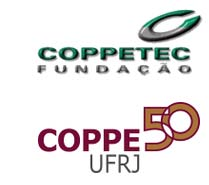
\includegraphics[width=40mm]{logo/coppetec50-logo.jpg}

\vfill%
\begin{center}
  {\GRANDE \raisebox{1.4ex}{} 
\includegraphics[width=80mm]{logo/projeto-EMMA-logo.jpg}} \\[10mm]
  %{\GRANDE \raisebox{1.4ex}{Projeto EMMA} } \\[10mm]
  {\Relatório de Interfaces de Usuários} \\[25mm]
  {\large \today}
  \vfill%
  %{\Large \today} \\[8mm]
\end{center}

\newpage%
%---------------------------------------------------------------------
\pagestyle{fancy}%
\thispagestyle{fancy}%
\renewcommand{\headrulewidth}  {0.4pt}%
\renewcommand{\footrulewidth}  {0.4pt}%
\lhead{\vspace*{-6mm}
\includegraphics[width=30mm]{logo/lead-logo.jpg}}%
\chead{\vspace*{-6mm}\raisebox{1.7ex}{} 
\includegraphics[width=25mm]{logo/projeto-EMMA-logo.jpg}}%
%\chead{\vspace*{-6mm}\raisebox{1.7ex}{Projeto EMMA}}%
\rhead{\sf\thepage}%
\lfoot{Relatório de Teste Experimental}%
\cfoot{}%
\rfoot{\sf [\hours] \quad \today}%
%---------------------------------------------------------------------

\tableofcontents



\section{Relatório de Usabilidade}

O Robô EMMA é uma solução para o processo de metalização in situ, isto é, o revestimento de pás no ambiente de turbina, 
diminuindo o tempo de manutenção e, consequentemente, de máquina parada. Esta pesquisa é divida em duas partes; a viabilidade 
técnica e execução. Como parte da viabilidade técnica, a pesquisa de interface de usuários do projeto EMMA propõe diretrizes 
para a elaboração da interface gráfica do sistema de controle do Robô EMMA. Este Relatório aborda os aspectos técnicos que 
dão embasamento para o design de interfaces do sistema e a caracterização de suas funcionalidades, assim como fundamentos 
teóricos que das interações entre homem e máquina.


\section{Objetivo}

O objetivo deste relatório é fundamentar os aspectos técnicos e teóricos que envolvem a interface de usuário do sistema de 
controle do robô EMMA com os seguintes tópicos: modelo de Interação humano-automação, modelagem do sistema, modelos conceitual 
de interface de usuários.

\section{Modelo de Interação}

Automação é um termo amplo, que pode ter muitos significados dependendo do
contexto em que está inserido. Neste estudo, entende-se por automação a realização de tarefas e atividades com a ação de máquinas, sem a interferência direta do humano 
no processo operacional. A interação humano-automação se dá em circunstâncias em que as pessoas podem: (1) especificar 
para a automação a tarefa (através de computador de algum tipo), objetivos e restrições e trade-offs ou trocas entre os 
objetivos e restrições; (2) controlar a automação para iniciar, parar ou modificar a tarefa automática de execução; e 
(3) receber a partir da informação de automação, energia, objetos físicos, ou substâncias.

Desta forma os aspectos que permeiam a interação humano-automatização envolvem tanto o homem quanto a máquina numa alimentação mútua, 
onde a idéia central é que o sistema fornece ao homem determinada informação, que a processa e realimenta o sistema com tal informação 
transformada, ou seja de acordo com as necessidades de uso do sistema. 
Um modelo que define a interação humano-automação de forma mais detalhada é chamado de OODA LOOP (Observation, Orientation, Decision, Action) 
(Thomas, 2001 apud Gikkas, 2013) que leva em consideração não só os processos de interação, mas também elementos (subjetivos e concretos) que 
interferem em cada uma das etapas. 

O OODA LOOP (fig. 1) é um esquema com uma série de ações cognitivas e motorasrequeridas de um operador/usuário para tomar decisões e executá-las 
durante a interação. Este esquema leva em consideração aspectos referentes ao usuário, como experiências prévias, aspectos culturais, informação 
dada ao usuário e de canais de atenção. A análise e consideração de todas essas variáveis torna-se essencial para que o usuário possa entender o 
que se passa durante a ação de um de um sistema automatizado e assim agir corretamente diante de cada situação. Da mesma forma, sinaliza a 
importância de estabelecer um perfil usuário baseado naqueles que usarão de forma direta ou indireta e também influenciarão em aspectos do projeto.

\begin{figure}[htp]
\begin{center}
  \includegraphics[width=figureWidth]{oodaLoop.jpg}
  \caption[labelInTOC]{figureCaption}
  \label{figureLabel}
\end{center}
\end{figure}
 

O esquema OODA LOOP também é aplicado para o funcionamento dos sistemas em si, levando em consideração as variáveis, cenários pré-determinados e 
leituras dos sensores para tomar as suas decisões. Durante a comunicação entre os usuários e o sistema, os modelos das duas partes estão diretamente 
interligados, uma vez que a falha de interpretação por parte dos sensores ou um feedback impreciso interfere diretamente nas ações do operador.
Ao observar o modelo acima (fig. 2), pode-se perceber que fatores humanos subjetivos e culturais são de suma importância para o bom desempenho 
das tarefas envolvendo elementos automatizados - uma vez que a interpretação dos estados do sistema e do funcionamento do mesmo está em função das 
experiências prévias do usuário, assim como antecedentes culturais relacionados à automatização. Diversos autores 
(Parasuraman & Sinderman, 2011; DEGANI, 2003; Thomas apud Gikkas, 2013) afirmam que um dos principais fatores que influenciam a 
interação Humano-Automatização são as experiências prévias dos usuários com este tipo de sistema. Na prática o modelo nos fornece elementos cognitivos 
(observação, orientação, decisão e ação) para compreender as escolhas do usuário a partir da leitura que o ambiente e seus dispositivos. Ademais, 
nos fornece aspectos relevantes a serem considerados tanto no processo de envolvimento de usuários no projeto e consequentemente no design centrado 
no usuário.


\section{Modelagem do Sistema}

A meta principal do sistema de controle robótico EMMA é a de realizar metalização in situ, isto é, o revestimento de pás no ambiente de turbina, 
diminuindo o tempo de manutenção e, consequentemente, de parada de máquinas.


\subsection{Requistos do Sistema}
É ter um manipulador robótica instalado no ambiente do circuito hidráulico onde o revestimento deve acontecer, incluindo os sensores para medições 
necessárias e as ferramentas para executar a tarefa.

\subsection{Problema}
\begin {enumerate}
  \item Determinar ás áreas a serem revestidas.
  \item Instalar o manipulador na posição correta para realizar o revestimento.
  \item Calcular e validar a posição instalada do manipulador.
  \item Calcular como o manipulador deve se mover para realizar a o
  revestimento.
  \item Executar o revestimento.
\end{enumerate}





\end{document}
